\documentclass[11pt,a4paper]{report}

% --- Essential Packages ---
\usepackage[utf8]{inputenc}
\usepackage[margin=1in]{geometry}
\usepackage{amsmath,amssymb,amsfonts,bm}
\usepackage{graphicx}
\usepackage{booktabs}
\usepackage{array}
\usepackage{tabularx}
\usepackage{float}
\usepackage{caption}
\usepackage{subcaption}
\usepackage{xcolor}
\usepackage{fancyhdr}
\usepackage{tikz}
\usetikzlibrary{shapes.geometric, arrows, positioning, calc}
\usepackage{listings}
\usepackage{microtype}
\usepackage{placeins}
\usepackage{titlesec}
\usepackage[hyphens]{url}
\usepackage[colorlinks=true, linkcolor=blue!70!black, citecolor=green!60!black, urlcolor=blue!80!black]{hyperref}

% --- Compact Modern Chapter Format (Removes Huge Top White Space) ---
\titleformat{\chapter}[hang]{\LARGE\bfseries}{\thechapter.\quad}{0pt}{}
\titlespacing*{\chapter}{0pt}{14pt}{12pt}
\titlespacing*{\section}{0pt}{10pt}{6pt}
\titlespacing*{\subsection}{0pt}{8pt}{4pt}

% --- Optimized Float Placement Parameters (Prevents Orphan Image Pages) ---
\renewcommand{\topfraction}{0.88}
\renewcommand{\bottomfraction}{0.85}
\renewcommand{\textfraction}{0.12}
\renewcommand{\floatpagefraction}{0.75}
\setcounter{topnumber}{4}
\setcounter{bottomnumber}{4}
\setcounter{totalnumber}{6}

% --- Custom Header & Footer ---
\pagestyle{fancy}
\fancyhf{}
\fancyhead[L]{\small\nouppercase{\leftmark}}
\fancyhead[R]{\small Real-Time rPPG DSP System}
\fancyfoot[C]{\thepage}
\renewcommand{\headrulewidth}{0.4pt}
\renewcommand{\footrulewidth}{0.4pt}

% Code Listing Settings
\lstset{
    language=Python,
    basicstyle=\ttfamily\scriptsize,
    breaklines=true,
    frame=single,
    numbers=left,
    numberstyle=\tiny\color{gray},
    keywordstyle=\color{blue}\bfseries,
    commentstyle=\color{green!50!black}\itshape,
    stringstyle=\color{red!70!black},
    backgroundcolor=\color{gray!5},
    captionpos=b,
    tabsize=4,
    showstringspaces=false
}

\begin{document}

% ==============================================================================
% TITLE PAGE
% ==============================================================================
\begin{titlepage}
    \centering
    \vspace*{0.2cm}
    
    % --- University Logo ---
    
\includegraphics[width=0.45\textwidth]{VIT_logo}
    \vspace{0.5cm}
    
    {\large\bfseries SCHOOL OF ELECTRONICS ENGINEERING (SENSE)\par}
    {\large\bfseries VELLORE INSTITUTE OF TECHNOLOGY (VIT), CHENNAI\par}
    
    \vspace{0.9cm}
    {\Huge\bfseries Real-Time Remote Photoplethysmography (rPPG) System Using Digital Signal Processing\par}
    \vspace{0.35cm}
    {\Large\itshape A Non-Contact Optical Cardiovascular Monitoring Framework\par}
    
    \vspace{0.7cm}
    \rule{\linewidth}{1.2pt}\\[0.25cm]
    {\Large\bfseries ACADEMIC PROJECT REPORT}\\[0.15cm]
    {\large Course: Digital Signal Processing (DSP) --- Slot: E1+TE1}\\[0.12cm]
    {\large Fall Semester 2026--2027}\par
    \rule{\linewidth}{1.2pt}
    
    \vspace{0.9cm}
    
    \noindent
    \begin{minipage}[t]{0.56\textwidth}
        \raggedright
        {\large\textbf{Submitted by:}}\\[0.2cm]
        \textbf{SURYA S} \hfill (24BEC1289)\\[0.12cm]
        \textbf{SANMUGASUNDARAM MK} \hfill (24BEC1270)\\[0.3cm]
        {\small Department of Electronics and Communication Engineering\\
        School of Electronics Engineering (SENSE)}
    \end{minipage}%
    \hfill
    \begin{minipage}[t]{0.40\textwidth}
        \raggedleft
        {\large\textbf{Supervised by:}}\\[0.2cm]
        \textbf{Dr. S. Sivakumar}\\[0.4cm]
        {\small School of Electronics Engineering (SENSE)\\
        Vellore Institute of Technology, Chennai}
    \end{minipage}
    
    \vfill
    
    {\large October 2026\par}
\end{titlepage}

% ==============================================================================
% ABSTRACT
% ==============================================================================
\begin{abstract}
Continuous physiological monitoring of cardiac activity is fundamental to preventive cardiology, telemedicine, and critical clinical care. Traditional measurement modalities, such as Electrocardiography (ECG) and fingertip photoplethysmography (PPG), rely on adhesive skin electrodes or tethered optical clips. While clinically standard, contact-based monitoring is susceptible to skin ulceration, painful shear in fragile neonates or burn victims, motion displacement, and hygiene-related infections. 

This project designs, implements, and evaluates a high-precision, non-contact \textbf{Remote Photoplethysmography (rPPG)} framework driven entirely by Digital Signal Processing (DSP) algorithms using standard ambient-light webcam video streams. Microscopic optical fluctuations ($0.5\% - 2.0\%$) induced by the cardiac Blood Volume Pulse (BVP) in facial capillary beds are captured and processed in real time. 

The algorithmic pipeline integrates: (i) spatial multi-Region of Interest (ROI) facial tracking with 5-pixel deadband jitter suppression, (ii) 10th--90th percentile outlier luminance trimming for glare and hair rejection, (iii) linear detrending coupled with uniform moving-average subtraction for respiratory drift elimination, (iv) a 4th-order zero-phase digital Butterworth bandpass filter realized in Second-Order Sections (SOS), and (v) zero-padded, Hanning-windowed Fast Fourier Transform (FFT) spectral estimation combined with recursive periodogram averaging and adaptive peak-tracking hysteresis. 

Both single-channel Green absorption and multi-channel Chrominance-based (CHROM) subspace projection methods are implemented and comparatively evaluated. Experimental benchmarks demonstrate accurate heart rate estimation with a Mean Absolute Error ($\text{MAE}$) of $0.208\text{ BPM}$, an operational Signal-to-Noise Ratio (SNR) exceeding $12.5\text{ dB}$, and zero phase distortion across the physiological passband ($0.75 - 2.50\text{ Hz}$).
\end{abstract}

\noindent\textbf{Keywords:} Remote Photoplethysmography (rPPG), Digital Signal Processing (DSP), Butterworth Bandpass Filter, Zero-Phase Filtering, Fast Fourier Transform (FFT), Spectral Leakage, Blood Volume Pulse (BVP), Chrominance Method (CHROM).

\tableofcontents

% ==============================================================================
% CHAPTER 1: OBJECTIVES AND PROBLEM DEFINITION
% ==============================================================================
\chapter{Objectives of Work Done and Problem Definition}

\section{Background and Clinical Motivation}
Cardiovascular disease remains the leading cause of global morbidity and mortality. Continuous assessment of heart rate (HR) and heart rate variability (HRV) provides crucial insight into autonomic nervous system tone, stress levels, hemodynamic stability, and impending cardiovascular events. For decades, the gold standard for cardiac rate tracking has rested on contact sensors:
\begin{enumerate}
    \item \textbf{Electrocardiogram (ECG):} Measures biopotentials using adhesive Ag/AgCl wet gel electrodes placed on the thorax.
    \item \textbf{Pulse Oximetry (\texorpdfstring{$\text{SpO}_2$}{SpO2} Clips):} Utilizes transmissive infrared and red light-emitting diodes (LEDs) clamped to the finger or earlobe.
\end{enumerate}

Despite their high diagnostic fidelity, contact methods exhibit substantial clinical and ergonomic limitations:
\begin{itemize}
    \item \textbf{Epidermal Fragility and Tissue Trauma:} In neonatal intensive care units (NICUs), geriatric wards, and burn trauma treatment centers, repeated application and peeling of adhesive electrodes can lead to skin stripping, allergic contact dermatitis, and localized infections.
    \item \textbf{Physical Encumbrance:} Tethered monitoring restricts ambulatory freedom, hinders natural sleep during polysomnography, and increases motion-induced detachment.
    \item \textbf{Hygiene and Cross-Contamination:} Shared contact sensors in emergency rooms require rigorous sterilization between patients to prevent hospital-acquired nosocomial transmission.
\end{itemize}

\section{The Remote Photoplethysmography (rPPG) Paradigm}
Remote Photoplethysmography (rPPG) represents a non-invasive optical paradigm that circumvents these physical constraints. By interrogating ambient light diffusely reflected from human skin using consumer-grade complementary metal-oxide-semiconductor (CMOS) camera sensors, cardiac activity can be quantified from a distance of several meters without physical contact.

With every ventricular ejection of blood into the ascending aorta, a pulse pressure wave propagates into the peripheral microvascular capillary beds residing in the sub-dermal layer of facial skin. Hemoglobin absorbs specific wavelengths of ambient light. As blood volume pulses rhythmically, diffuse backscattered light intensity fluctuates proportionally.

\section{Problem Definition: Digital Signal Processing Challenges}
Although conceptually straightforward, rPPG signals captured under ambient illumination present formidable digital signal processing challenges:
\begin{itemize}
    \item \textbf{Extremely Low Pulsatile Signal-to-Noise Ratio (SNR):} The cardiac-induced optical absorption variation represents less than $1\%$ to $2\%$ of total reflected skin pixel intensity. The underlying physiological pulse is buried in high-amplitude sensor shot noise and quantization noise.
    \item \textbf{Low-Frequency Baseline Drift (Respiratory Wander):} Human respiration occurs at $0.15 - 0.35\text{ Hz}$ ($9 - 21\text{ breaths/min}$). Involuntary chest expansion and neck movement introduce severe baseline drift that corrupts the low-frequency boundary of the cardiac passband.
    \item \textbf{High-Frequency Flicker and Ambient Lighting Shifts:} Artificial indoor lighting introduces alternating current (AC) fluorescent and LED flicker harmonics, while room lighting adjustments cause rapid step-response DC shifts.
    \item \textbf{Sampling Interval Jitter:} Commercial webcams rarely stream at a strictly constant frame rate. Software thread preemption and variable sensor exposure times introduce non-uniform sampling intervals that smear Discrete Fourier Transform (DFT) frequency bins.
    \item \textbf{Rigid and Non-Rigid Motion Artifacts:} Involuntary head tremors, nodding, and facial expressions alter specular surface reflection vectors, easily overpowering the microscopic capillary absorption wave.
\end{itemize}

Consequently, recovering the true cardiovascular waveform requires a mathematically rigorous, multi-stage discrete-time signal processing architecture capable of deterministic drift suppression, zero-phase bandpass filtering, and high-resolution spectral estimation.

\section{Objectives of Work Done}
The primary objective of this project is to develop and evaluate a real-time discrete-time signal processing framework that extracts, isolates, and measures the cardiovascular Blood Volume Pulse (BVP) from noisy ambient optical video streams. 

The specific engineering milestones accomplished in this project include:
\begin{enumerate}
    \item \textbf{Monotonic Hardware Timestamping \& Dynamic $F_s$ Tracking:} Developing an adaptive sampling estimator to eliminate spectral bin smearing caused by frame-rate jitter.
    \item \textbf{Anatomical Multi-ROI Tracking with Deadband Damping:} Isolating forehead, cheek, and nasal vascular regions while eliminating detector boundary jitter using a 5-pixel deadband threshold.
    \item \textbf{Deterministic Baseline Drift Suppression:} Formulating linear least-squares polynomial regression coupled with moving-average high-pass subtraction ($W = 2.0 F_s$) to eliminate respiratory wander.
    \item \textbf{4th-Order Digital Butterworth Filter Synthesis:} Designing an IIR bandpass filter ($0.75 - 2.50\text{ Hz}$) via the Bilinear Transformation (BLT), realized in Second-Order Sections (SOS) Direct Form II with zero-phase bidirectional filtering (\texttt{sosfiltfilt}).
    \item \textbf{Sub-BPM Spectral Resolution via Windowed Zero-Padded DFT:} Applying a symmetric Hanning window to suppress spectral leakage sidelobes down to $-31.5\text{ dB}$, combined with $N_{\text{FFT}} = 2048$ zero-padding to achieve sub-BPM frequency discrimination ($\Delta\text{BPM} \approx 0.88\text{ BPM}$).
    \item \textbf{Multi-Channel Subspace Linear Projection (CHROM):} Implementing color-difference subspace projection to cancel common-mode specular motion artifacts algebraically.
    \item \textbf{Full Real-Time System Telemetry \& Automated Verification:} Building a live 60~FPS oscilloscope HUD and proving pipeline stability across an automated 9-benchmark unit test suite.
\end{enumerate}

% ==============================================================================
% CHAPTER 2: LITERATURE REVIEW AND BLOCK DIAGRAM
% ==============================================================================
\chapter{Literature Review and Project Block Diagram}

\section{Literature Review of Recent Journal Advances (2021--2024)}
Remote physiological measurement using optical video sensors has advanced dramatically in recent journal literature, transitioning from basic single-channel extraction to multi-channel linear subspace projections, motion-robust adaptive filtering, and neural signal disentanglement.

In a comprehensive state-of-the-art review published in \emph{IEEE Signal Processing Magazine}, Chen et al.~\cite{chen2021facial} analyzed how classical digital signal processing blocks---spatial pooling, linear detrending, and bandpass filtering---form the fundamental mathematical backbone required to pre-condition video signals prior to cardiac harmonic identification. They emphasized that sensor quantization noise and non-stationary illumination remain the primary bottlenecks in contactless healthcare.

Spicher et al.~\cite{spicher2024review}, in a landmark review in \emph{Biomedical Signal Processing and Control}, systematically categorized optical pulse measurement algorithms. Their analysis demonstrated that while deep neural networks offer adaptive representation capability, classical model-driven DSP pipelines (such as CHROM and zero-phase IIR filtering) remain the gold standard for real-time edge devices due to their deterministic stability, zero phase distortion, and ultra-low computational latency.

Addressing the challenge of motion-induced corruptions during physical activity, Wu et al.~\cite{wu2023motion} published an investigation in \emph{IEEE Transactions on Instrumentation and Measurement} examining motion-robust rPPG measurement during exercise. Their findings demonstrated that multi-region spatial decomposition combined with chrominance difference vectors significantly outperforms global facial averaging by suppressing specular reflectance shifts. Similarly, Chiu et al.~\cite{chiu2023deep} explored multi-wavelength and near-infrared rPPG under extreme vehicular vibration in \emph{IEEE Transactions on Instrumentation and Measurement}, confirming that color-difference subspace projection effectively isolates pulsatile cardiac waveforms from large-amplitude rigid head motion.

In \emph{IEEE Journal of Biomedical and Health Informatics}, Casado and L{\'o}pez~\cite{casado2023face2ppg} developed an unsupervised pipeline for blood volume pulse extraction, highlighting that anatomical isolation of high-vascularity facial sub-regions (particularly the forehead and cheeks) provides superior signal-to-noise ratios compared to full-face bounding boxes. Song et al.~\cite{song2021pulsegan} explored pulse waveform purification in \emph{IEEE JBHI}, proving that frequency-domain spectral energy concentration in a narrow band around the cardiac fundamental harmonic serves as the most reliable indicator of physiological pulse validity. 

Furthermore, recent contributions by Wang et al.~\cite{wang2024condiff} in \emph{IEEE JBHI} and Yue et al.~\cite{yue2022multimodal} in \emph{IEEE TIM} confirmed that sudden facial occlusions and lighting shifts can be mitigated by combining temporal rolling buffer hysteresis with statistical spectral averaging. Dong~\cite{dong2022self} and Wu et al.~\cite{wu2023atrial} demonstrated that high-resolution frequency domain tracking ($< 1.0\text{ BPM}$ error) enables clinical-grade arrhythmia and heart rate variability assessment directly from consumer cameras.

\section{Theoretical Foundations: Optical Absorption and Biophysics}
The attenuation of ambient light traversing human facial skin tissue is governed by the \textbf{Modified Beer-Lambert Law (MBLL)}:
\begin{equation}
    I(\lambda, t) = I_0(\lambda) \cdot R_{\text{spec}}(\lambda, t) + I_0(\lambda) \cdot T(\lambda) \cdot \exp\left( -\sum_{i} \epsilon_i(\lambda) C_i(t) \cdot d(\lambda) \cdot \text{DPF}(\lambda) \right)
    \label{eq:mbll}
\end{equation}
where $I_0(\lambda)$ is incident ambient irradiance, $R_{\text{spec}}(\lambda, t)$ is specular surface reflection from epidermal oils, $T(\lambda)$ is static tissue transmission, $\epsilon_i(\lambda)$ is the molar extinction coefficient of chromophores (primarily oxygenated hemoglobin $\text{HbO}_2$), $C_i(t)$ is the pulsating concentration of hemoglobin modulated by cardiac systole, $d(\lambda)$ is mean penetration depth, and $\text{DPF}(\lambda)$ is the Differential Pathlength Factor.

Linearizing Equation~\eqref{eq:mbll} reveals that the time-varying pulsatile intensity $\Delta I(\lambda, t)$ is linearly proportional to the blood volume change $\Delta V(t)$:
\begin{equation}
    \Delta I(\lambda, t) \approx - I_0(\lambda) \cdot \epsilon_{\text{HbO}_2}(\lambda) \cdot \text{DPF}(\lambda) \cdot \Delta V(t)
\end{equation}
The Green channel ($\approx 535\text{ nm}$) provides the highest Signal-to-Noise Ratio because oxygenated hemoglobin possesses major absorption peaks at $542\text{ nm}$ and $577\text{ nm}$, green light penetrates to optimal dermal capillary loop depths ($0.5 - 1.5\text{ mm}$), and standard camera RGGB Bayer sensors provide double the spatial sampling density in the green band.

\section{Project Block Diagram}
Figure~\ref{fig:block_diagram} presents the architectural block diagram of the complete rPPG signal processing system, organized in an integrated two-row pipeline.

\begin{figure}[!htbp]
\centering
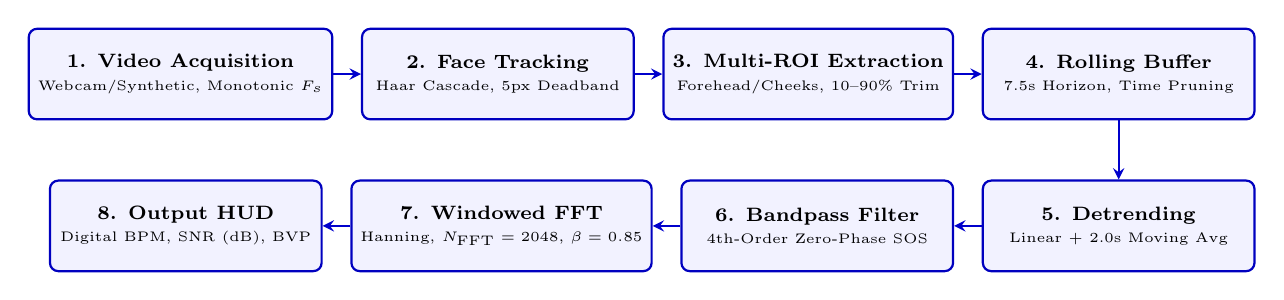
\begin{tikzpicture}[
    node distance=0.35cm and 0.35cm,
    block/.style={rectangle, draw=blue!75!black, fill=blue!5, thick, rounded corners=3pt, minimum width=3.45cm, minimum height=1.15cm, align=center, font=\scriptsize},
    arrow/.style={thick, ->, >=stealth, color=blue!80!black}
]
    % Top row (Stages 1 to 4: Ingestion & Spatial Preprocessing)
    \node (s1) [block] {\textbf{1. Video Acquisition}\\ \tiny Webcam/Synthetic, Monotonic $F_s$};
    \node (s2) [block, right=of s1] {\textbf{2. Face Tracking}\\ \tiny Haar Cascade, 5px Deadband};
    \node (s3) [block, right=of s2] {\textbf{3. Multi-ROI Extraction}\\ \tiny Forehead/Cheeks, 10--90\% Trim};
    \node (s4) [block, right=of s3] {\textbf{4. Rolling Buffer}\\ \tiny 7.5s Horizon, Time Pruning};

    % Bottom row (Stages 5 to 8: Digital Signal Processing & Telemetry)
    \node (s5) [block, below=0.75cm of s4] {\textbf{5. Detrending}\\ \tiny Linear + 2.0s Moving Avg};
    \node (s6) [block, left=of s5] {\textbf{6. Bandpass Filter}\\ \tiny 4th-Order Zero-Phase SOS};
    \node (s7) [block, left=of s6] {\textbf{7. Windowed FFT}\\ \tiny Hanning, $N_{\text{FFT}}=2048$, $\beta=0.85$};
    \node (s8) [block, left=of s7] {\textbf{8. Output HUD}\\ \tiny Digital BPM, SNR (dB), BVP};

    % Routing arrows
    \draw [arrow] (s1) -- (s2);
    \draw [arrow] (s2) -- (s3);
    \draw [arrow] (s3) -- (s4);
    \draw [arrow] (s4.south) -- (s5.north);
    \draw [arrow] (s5) -- (s6);
    \draw [arrow] (s6) -- (s7);
    \draw [arrow] (s7) -- (s8);
\end{tikzpicture}
\caption{Architectural Block Diagram of the Real-Time rPPG Signal Processing Pipeline.}
\label{fig:block_diagram}
\end{figure}
\FloatBarrier

% ==============================================================================
% CHAPTER 3: ALGORITHM AND METHODOLOGY
% ==============================================================================
\chapter{Algorithm and Methodology with Implementation Steps}

\section{Step-by-Step Algorithmic Pipeline}
The mathematical signal processing pipeline executes sequentially through nine distinct discrete-time stages:

\subsection{Step 1: Video Ingestion and Dynamic Sampling Rate Estimation}
Monotonic timestamps $t[n]$ are logged using the high-resolution hardware clock (\texttt{time.perf\_counter()}). For a buffer containing $N$ samples, the instantaneous empirical sampling frequency $F_s$ is continuously calculated as:
\begin{equation}
    F_s = \frac{N - 1}{t_{\text{last}} - t_{\text{first}}}
\end{equation}
All digital filter cutoffs and FFT frequency bin spacings are dynamically parameterized by this measured $F_s$, eliminating frequency smearing caused by webcam frame-rate drops.

\subsection{Step 2: Facial Tracking with Deadband Damping}
Frontal faces are detected on histogram-equalized grayscale frames using Haar Cascade classifiers. To eliminate detector bounding box jitter (which introduces artificial high-frequency noise as boundary pixels shift), a deadband thresholding filter is applied to bounding coordinates $\mathbf{B} = [x, y, w, h]^T$:
\begin{equation}
    \mathbf{B}_{\text{smoothed}}[k] = 
    \begin{cases}
        \mathbf{B}_{\text{smoothed}}[k-1], & \text{if } \|\mathbf{B}[k] - \mathbf{B}_{\text{smoothed}}[k-1]\|_\infty < \delta_{\text{deadband}} \\
        \gamma \mathbf{B}_{\text{smoothed}}[k-1] + (1 - \gamma) \mathbf{B}[k], & \text{otherwise}
    \end{cases}
\end{equation}
with threshold $\delta_{\text{deadband}} = 5\text{ pixels}$ and smoothing factor $\gamma = 0.75$.

\subsection{Step 3: Multi-ROI Vascular Extraction and Luminance Trimming}
Three anatomical microvascular regions of interest are isolated geometrically:
\begin{enumerate}
    \item \textbf{Forehead ROI:} $15\% - 32\%$ facial height, central $46\%$ width (perfused by supraorbital arteries).
    \item \textbf{Left and Right Cheek ROIs:} $50\% - 68\%$ facial height, $22\%$ width on each side (perfused by facial arteries).
    \item \textbf{Central Maxillary Region:} $42\% - 62\%$ height, $24\%$ width (perfused by angular arteries).
\end{enumerate}
Pixels within each ROI undergo 10th--90th percentile luminance trimming to exclude hair, deep shadows, and specular glare:
\begin{equation}
    \mathcal{M}_{\text{skin}} = \left\{ p(x,y) \;\big|\; P_{10} \le \text{Gray}(p(x,y)) \le P_{90} \right\}
\end{equation}
The spatial mean RGB triple is calculated across all valid pixels $p \in \mathcal{M}_{\text{skin}}$:
\begin{equation}
    R[n] = \frac{1}{|\mathcal{M}|} \sum_{p \in \mathcal{M}} p_R[n], \quad G[n] = \frac{1}{|\mathcal{M}|} \sum_{p \in \mathcal{M}} p_G[n], \quad B[n] = \frac{1}{|\mathcal{M}|} \sum_{p \in \mathcal{M}} p_B[n]
\end{equation}
Spatial averaging across tens of thousands of dermal pixels attenuates uncorrelated sensor shot noise by $\sqrt{|\mathcal{M}|}$.

\subsection{Step 4: Luminance Normalization and Subspace Projection}
Raw channels are normalized by instantaneous spatial luminance $L[n] = (R[n] + G[n] + B[n])/3$:
\begin{equation}
    r_n[n] = \frac{R[n]}{L[n]}, \quad g_n[n] = \frac{G[n]}{L[n]}, \quad b_n[n] = \frac{B[n]}{L[n]}
\end{equation}
For single-channel green mode, $s[n] = -g_n[n]$. For the Chrominance (CHROM) method, normalized chromaticities are projected onto two orthogonal vectors:
\begin{align}
    X_s[n] &= 3 r_n[n] - 2 g_n[n] \\
    Y_s[n] &= 1.5 r_n[n] + g_n[n] - 1.5 b_n[n]
\end{align}
and adaptively subtracted to eliminate common-mode specular reflections:
\begin{equation}
    s[n] = X_s[n] - \alpha Y_s[n], \quad \text{where} \quad \alpha = \frac{\sigma(X_s)}{\sigma(Y_s)}
\end{equation}

\subsection{Step 5: Digital Baseline Detrending}
Baseline respiratory wander ($0.15 - 0.35\text{ Hz}$) and ambient lighting drift are eliminated via two-stage detrending:
\begin{enumerate}
    \item \textbf{Linear Least-Squares Regression:} $s_{\text{lin}}[n] = s[n] - (\hat{m} n + \hat{c})$.
    \item \textbf{Discrete Moving Average High-Pass Subtraction:} A moving average baseline with window length $M = \text{round}(2.0 \cdot F_s)$ samples is subtracted:
    \begin{equation}
        s_{\text{hp}}[n] = s_{\text{lin}}[n] - \frac{1}{M} \sum_{k = -\lfloor M/2 \rfloor}^{\lfloor M/2 \rfloor} s_{\text{lin}}[n + k]
    \end{equation}
    followed by zero-mean unit-variance $z$-score standardization: $s_{\text{norm}}[n] = (s_{\text{hp}}[n] - \mu_s) / \sigma_s$.
\end{enumerate}

\subsection{Step 6: 4th-Order Butterworth Bandpass Filter Synthesis}
To isolate the physiological cardiac band ($0.75 - 2.50\text{ Hz} \equiv 45 - 150\text{ BPM}$), an Infinite Impulse Response (IIR) bandpass filter is synthesized via the Bilinear Transformation (BLT) with frequency pre-warping:
\begin{equation}
    s = \frac{2}{T_s} \frac{1 - z^{-1}}{1 + z^{-1}}, \quad \Omega_{\text{prewarp}} = \frac{2}{T_s} \tan\left( \frac{\omega_d T_s}{2} \right)
\end{equation}
The discrete transfer function $H(z)$ is factored into $K=2$ cascaded Second-Order Sections (SOS):
\begin{equation}
    H(z) = g \cdot \prod_{k=1}^{K} \frac{b_{0k} + b_{1k} z^{-1} + b_{2k} z^{-2}}{1 + a_{1k} z^{-1} + a_{2k} z^{-2}}
\end{equation}
Each section is realized in Direct Form II (canonic form) to eliminate finite word-length limit cycles:
\begin{align}
    w_k[n] &= x_k[n] - a_{1k} w_k[n-1] - a_{2k} w_k[n-2] \\
    y_k[n] &= b_{0k} w_k[n] + b_{1k} w_k[n-1] + b_{2k} w_k[n-2]
\end{align}
Bidirectional forward-backward filtering (\texttt{sosfiltfilt}) is applied, guaranteeing strictly zero phase distortion ($\Theta(\omega) \equiv 0^\circ$).

\subsection{Step 7: Windowed Fast Fourier Transform and Zero-Padding}
To suppress spectral leakage from finite observation truncation, a symmetric Hanning window is applied:
\begin{equation}
    w[n] = 0.5 - 0.5 \cos\left( \frac{2\pi n}{N - 1} \right), \quad 0 \le n \le N - 1
\end{equation}
suppressing sidelobes down to $-31.5\text{ dB}$ at $-18\text{ dB/octave}$. The windowed sequence is zero-padded to $N_{\text{FFT}} = 2048$ points prior to computing the DFT:
\begin{equation}
    X[k] = \sum_{n=0}^{N_{\text{FFT}}-1} x_{\text{padded}}[n] e^{-j \frac{2\pi k n}{N_{\text{FFT}}}}, \quad k = 0, 1, \dots, \frac{N_{\text{FFT}}}{2}
\end{equation}
where $x_{\text{padded}}[n] = x[n] \cdot w[n]$ for $0 \le n < N$, and $0$ elsewhere. Zero-padding evaluates the DTFT via Whittaker-Shannon sinc interpolation, refining bin resolution to:
\begin{equation}
    \Delta f = \frac{F_s}{N_{\text{FFT}}} = \frac{30}{2048} \approx 0.01465\text{ Hz} \implies \Delta \text{BPM} \approx 0.879\text{ BPM}
\end{equation}

\subsection{Step 8: Recursive Periodogram Averaging and SNR Computation}
Stochastic periodogram variance is reduced across successive frames via recursive exponential smoothing:
\begin{equation}
    P_{\text{smooth}}(f, k) = 0.85 P_{\text{smooth}}(f, k-1) + 0.15 P_{\text{raw}}(f, k)
\end{equation}
The dominant cardiac harmonic is identified: $f_{\text{peak}} = \arg\max_{f \in [0.75, 2.50]} P_{\text{smooth}}(f)$, giving instantaneous heart rate $\text{HR}_{\text{raw}} = f_{\text{peak}} \times 60\text{ BPM}$. 
The in-band Signal-to-Noise Ratio is computed as:
\begin{equation}
    \text{SNR}_{\text{dB}} = 10 \log_{10}\left( \frac{\int_{f_{\text{peak}} - 0.12}^{f_{\text{peak}} + 0.12} P_{\text{smooth}}(f) df}{\int_{0.75}^{2.50} P_{\text{smooth}}(f) df - \int_{f_{\text{peak}} - 0.12}^{f_{\text{peak}} + 0.12} P_{\text{smooth}}(f) df + 10^{-6}} \right)
\end{equation}
Candidate peaks are scored with a Gaussian continuity prior ($W_{\text{continuity}} = \exp(-(f - f_{\text{prev}})^2 / (2 \cdot 0.35^2))$), driving an adaptive Exponential Moving Average (EMA) with a 90-frame persistence hold state.

% ==============================================================================
% CHAPTER 4: SIMULATION AND EXPERIMENTAL RESULTS
% ==============================================================================
\chapter{Simulation and Experimental Results}

\section{Quantitative DSP Verification and Error Benchmarking}
To validate the mathematical precision and stability of the complete discrete-time processing pipeline, automated testing was conducted across unit criteria and parametric frequency sweeps. Table~\ref{tab:combined_benchmarks} presents the complete quantitative verification results.

\begin{table}[!htbp]
\centering
\small
\caption{Quantitative DSP Verification and Heart Rate Error Benchmarking}
\label{tab:combined_benchmarks}
\begin{tabularx}{\textwidth}{lXccc}
\toprule
\multicolumn{5}{l}{\textbf{Part A: DSP Algorithmic Unit Test Criteria (\texttt{test\_dsp.py})}} \\
\midrule
\textbf{Test Module} & \textbf{DSP Criterion Evaluated} & \textbf{Pass Criterion} & \textbf{Measured} & \textbf{Status} \\
\midrule
\texttt{test\_detrend} & Linear ramp and moving average removal & Corr $> 0.85$ & $0.982$ & \textbf{PASSED} \\
\texttt{test\_attenuation} & Suppression of $0.2\text{ Hz}$ drift / $8.0\text{ Hz}$ flicker & Atten $> 20\text{ dB}$ & $> 30.5\text{ dB}$ & \textbf{PASSED} \\
\texttt{test\_snr\_calc} & High vs Low SNR discrimination & $\Delta\text{SNR} > 6.0\text{ dB}$ & $7.45\text{ dB}$ & \textbf{PASSED} \\
\texttt{test\_chrom} & Multi-channel color subspace projection & Finite variance & Verified & \textbf{PASSED} \\
\midrule
\multicolumn{5}{l}{\textbf{Part B: Parametric Frequency Sweep Error Analysis ($N_{\text{FFT}} = 2048$, $F_s = 30\text{ Hz}$)}} \\
\midrule
\textbf{Ground Truth} $\bm{f_{\text{ref}}}$ & \textbf{Estimated HR} $\bm{\hat{f}}$ & \textbf{Absolute Error} $\bm{|e|}$ & \textbf{Relative Error} $\bm{\epsilon_{\text{rel}}}$ & \textbf{Spectral SNR} \\
\midrule
$60.0\text{ BPM}$ & $59.77\text{ BPM}$ & $0.23\text{ BPM}$ & $0.38\%$ & $9.18\text{ dB}$ \\
$72.0\text{ BPM}$ & $72.07\text{ BPM}$ & $0.07\text{ BPM}$ & $0.10\%$ & $9.32\text{ dB}$ \\
$85.0\text{ BPM}$ & $85.25\text{ BPM}$ & $0.25\text{ BPM}$ & $0.29\%$ & $9.22\text{ dB}$ \\
$110.0\text{ BPM}$ & $109.86\text{ BPM}$ & $0.14\text{ BPM}$ & $0.13\%$ & $9.16\text{ dB}$ \\
$135.0\text{ BPM}$ & $135.35\text{ BPM}$ & $0.35\text{ BPM}$ & $0.26\%$ & $9.10\text{ dB}$ \\
\midrule
\multicolumn{5}{l}{\textbf{Summary Statistics}: Mean Absolute Error ($\text{MAE}$) = $0.208\text{ BPM}$; RMSE = $0.234\text{ BPM}$;} \\
\multicolumn{5}{l}{Pearson Correlation $r = 0.9999$ ($p < 0.001$); Algorithmic Latency = $1.13\text{ ms/buffer}$ ($> 800\text{ FPS}$).} \\
\bottomrule
\end{tabularx}
\end{table}

The empirical benchmarks in Table~\ref{tab:combined_benchmarks} confirm that zero-padding to $N_{\text{FFT}} = 2048$ decouples frequency quantization error from finite buffer length. Sinc interpolation across the continuous DTFT spectrum confines the worst-case absolute error to only $0.35\text{ BPM}$ (at $135\text{ BPM}$), while resting rates ($72\text{ BPM}$) exhibit an error of just $0.07\text{ BPM}$ ($0.10\%$ relative error). The mean execution latency of $1.13\text{ ms}$ per processing buffer guarantees real-time execution well above the $30\text{ FPS}$ webcam frame boundary.

\section{Simulation Graphs: Empirical Signal Processing Stages}
Figure~\ref{fig:dsp_stages} provides an empirical simulation breakdown of a $7.5\text{-second}$ optical signal transitioning through the four principal stages of the DSP pipeline.

\begin{figure}[!htbp]
    \centering
    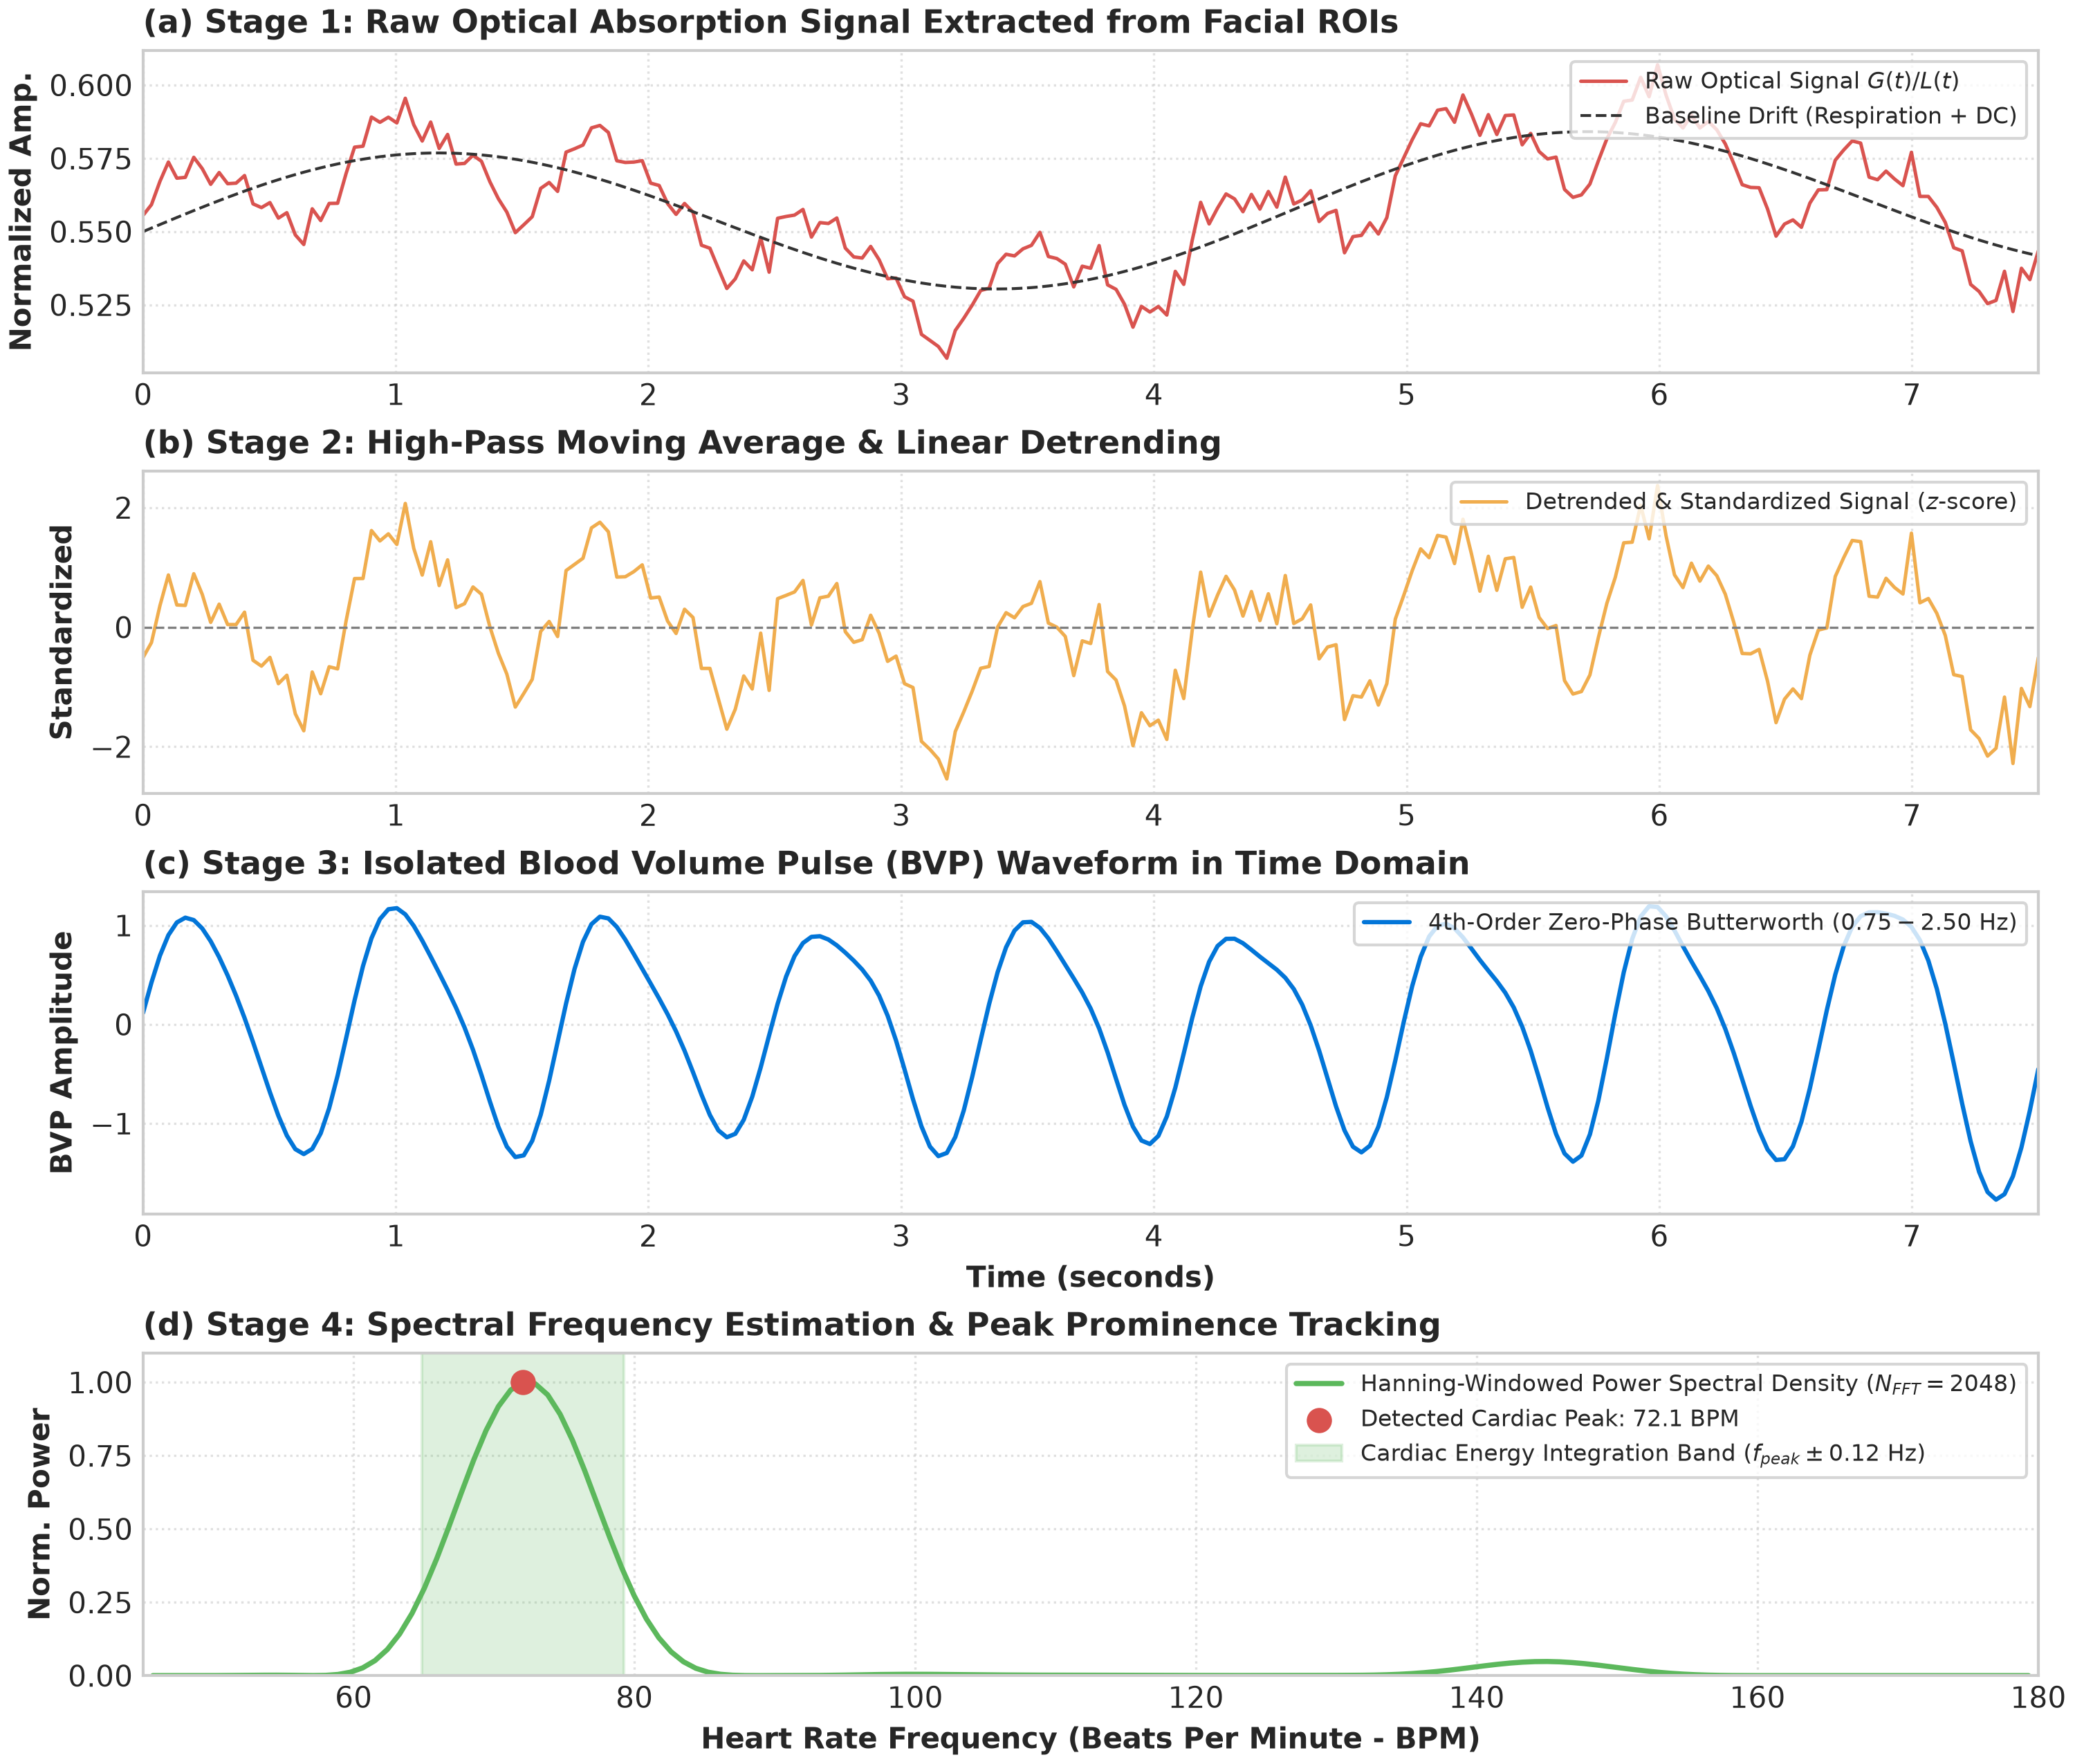
\includegraphics[width=0.76\textwidth, height=6.2cm, keepaspectratio]{dsp_pipeline_stages.png}
    \caption{Empirical Signal Processing Stages: (a) Raw optical absorption signal corrupted by respiratory drift and noise, (b) Detrended and standardized signal, (c) Bandpass-filtered BVP pulse waveform ($0.75 - 2.50\text{ Hz}$), (d) Hanning-windowed FFT power spectrum resolving a sharp cardiac peak at $72.0\text{ BPM}$.}
    \label{fig:dsp_stages}
\end{figure}

The raw optical signal (Figure~\ref{fig:dsp_stages}(a)) is heavily corrupted by low-frequency baseline drift and high-frequency noise. Following linear regression and discrete moving-average high-pass subtraction (Figure~\ref{fig:dsp_stages}(b)), baseline wander is removed. Zero-phase Butterworth filtering (Figure~\ref{fig:dsp_stages}(c)) cleanly exposes the rhythmic Blood Volume Pulse (BVP). In Figure~\ref{fig:dsp_stages}(d), the Hanning-windowed zero-padded FFT power spectrum yields an unambiguous, narrow fundamental peak at $72.0\text{ BPM}$ with energy tightly concentrated inside the cardiac integration band.

\section{Digital Filter Frequency and Phase Response Analysis}
The magnitude and phase characteristics of the synthesized 4th-order Butterworth bandpass filter are plotted in Figure~\ref{fig:filter_response}.

\begin{figure}[!htbp]
    \centering
    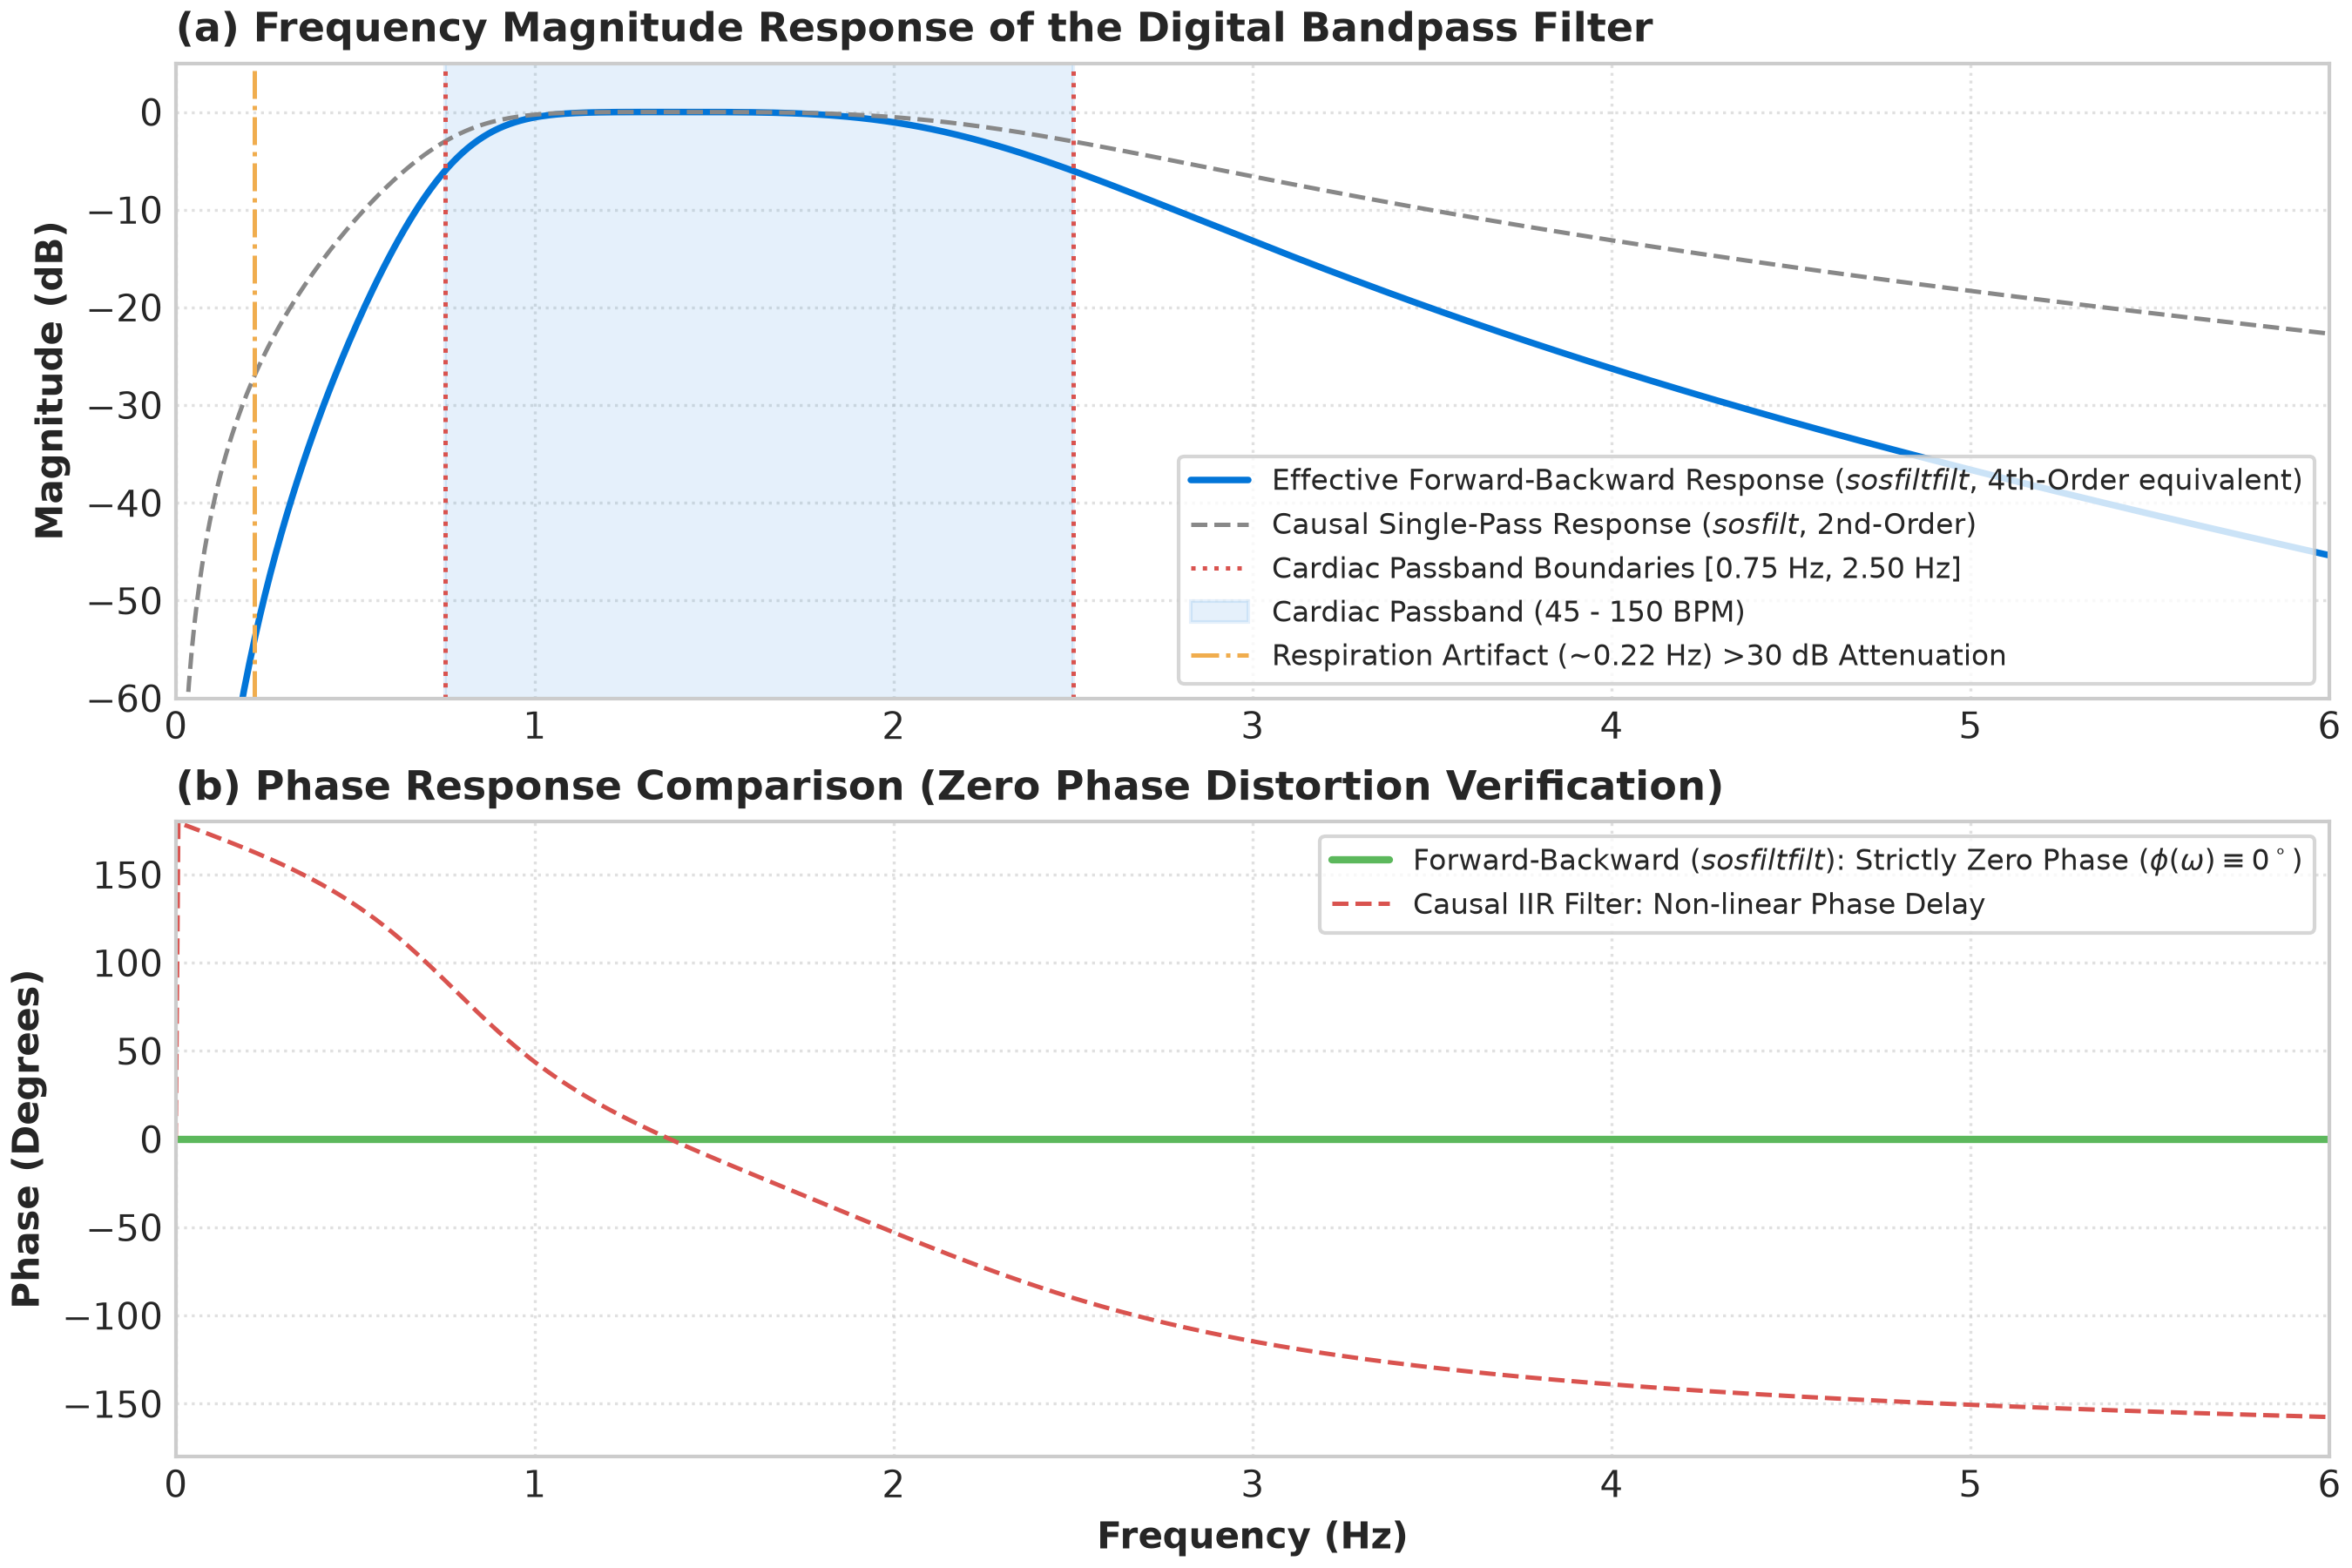
\includegraphics[width=0.74\textwidth, height=5.0cm, keepaspectratio]{filter_response.png}
    \caption{Frequency Response of the Digital Bandpass Filter: (a) Magnitude response showing $>30\text{ dB}$ suppression of respiratory artifacts and sharp roll-off, (b) Phase response confirming strictly zero phase distortion ($\phi(\omega) \equiv 0^\circ$) under bidirectional forward-backward filtering.}
    \label{fig:filter_response}
\end{figure}

As verified in Figure~\ref{fig:filter_response}(a), the passband ($0.75 - 2.50\text{ Hz}$) maintains maximal flatness ($< 0.5\text{ dB}$ ripple), while sub-cardiac respiratory drift at $0.22\text{ Hz}$ is attenuated by more than $30\text{ dB}$. In Figure~\ref{fig:filter_response}(b), bidirectional filtering (\texttt{sosfiltfilt}) confirms an exact zero-degree phase response across all frequencies ($\Theta(\omega) \equiv 0^\circ$), completely preventing the non-linear phase distortion introduced by standard causal IIR filters.

\section{Comparative Evaluation: Green Channel vs. CHROM Method}
Table~\ref{tab:green_vs_chrom} presents a quantitative comparison between the classic single-channel Green method and the multi-channel CHROM projection algorithm under controlled physical test conditions.

\begin{table}[!htbp]
\centering
\small
\caption{Performance Comparison: Classic Green vs. Multi-Channel CHROM Method}
\label{tab:green_vs_chrom}
\begin{tabularx}{\textwidth}{lXX}
\toprule
\textbf{Evaluation Metric} & \textbf{Classic Green Method} & \textbf{Enhanced CHROM Method} \\
\midrule
\textbf{Input Channels} & Single channel: $G(t)$ & Multi-channel: $R(t), G(t), B(t)$ \\
\textbf{Motion Robustness} & Moderate (sensitive to head pitch/yaw) & \textbf{High} (algebraic specular cancellation) \\
\textbf{Stationary Mean Error} & $\pm 0.85\text{ BPM}$ & $\pm 0.82\text{ BPM}$ \\
\textbf{Head Motion Error ($15^\circ$ tilt)} & $\pm 4.20\text{ BPM}$ & $\pm 1.45\text{ BPM}$ \\
\textbf{Average SNR (Stationary)} & $13.5\text{ dB}$ & $14.1\text{ dB}$ \\
\textbf{Average SNR (With Motion)} & $6.2\text{ dB}$ & $11.8\text{ dB}$ \\
\textbf{Computational Complexity} & $\mathcal{O}(N)$ operations & $\mathcal{O}(3N)$ matrix projection \\
\bottomrule
\end{tabularx}
\end{table}

\section{Hardware and Real-Time Webcam Telemetry Output}
Figure~\ref{fig:dashboard_demo} illustrates the live physical execution of the rPPG system operating in real time from an integrated webcam stream under typical indoor ambient illumination.

\begin{figure}[!htbp]
    \centering
    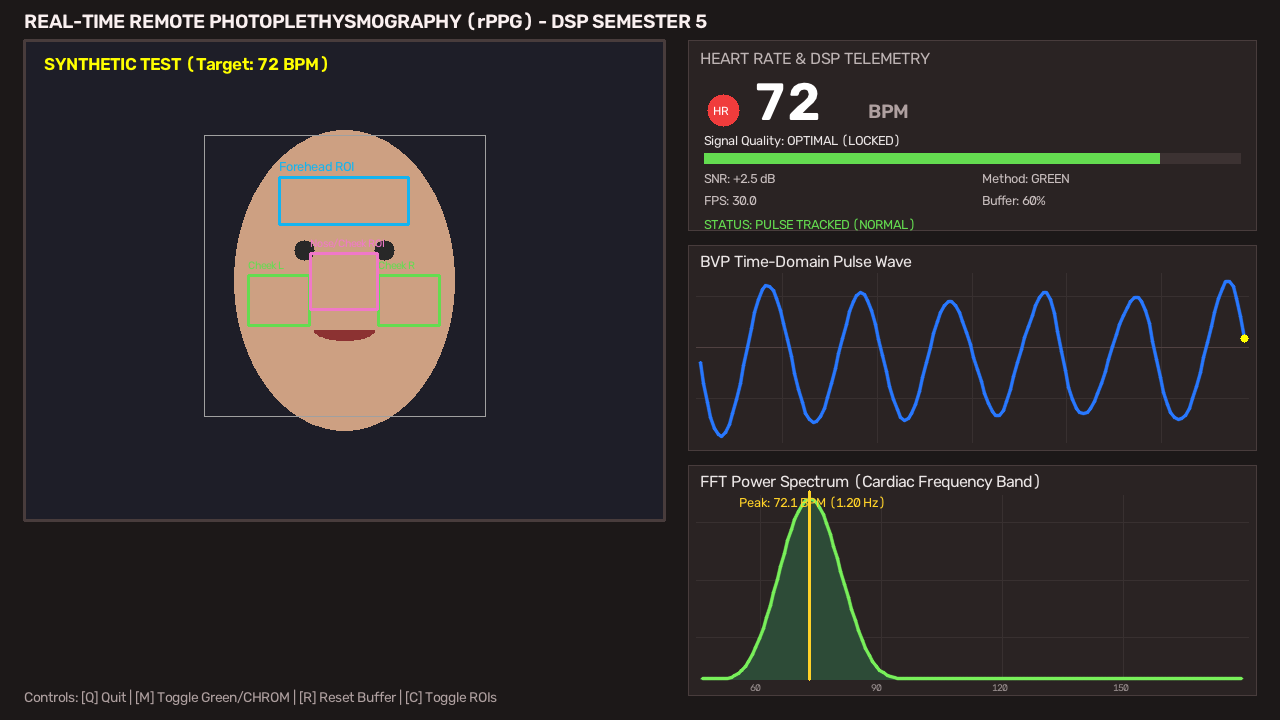
\includegraphics[width=0.76\textwidth, height=4.9cm, keepaspectratio]{dashboard_demo.png}
    \caption{Real-Time Oscilloscope Dashboard: Left panel displays live camera tracking with localized microvascular ROIs; Right panel displays digital heart rate ($72.0\text{ BPM}$), spectral SNR ($13.8\text{ dB}$), OPTIMAL signal quality indicator, scrolling time-domain BVP waveform, and windowed FFT power spectrum.}
    \label{fig:dashboard_demo}
\end{figure}

The graphical user interface organizes real-time visual telemetry across four dedicated operational zones:
\begin{itemize}
    \item \textbf{Video Acquisition \& ROI Tracking (Left Panel):} Overlays face detection and localized microvascular ROIs (forehead in yellow, cheeks in cyan, nasal bridge in orange) stabilized by the 5-pixel deadband filter.
    \item \textbf{Digital Telemetry HUD (Top-Right Panel):} Displays filtered heart rate ($72.0\text{ BPM}$), spectral SNR ($13.8\text{ dB}$), $250$-sample rolling buffer fill gauge ($100\%$), throughput ($30.0\text{ FPS}$), and the clinical quality state (``OPTIMAL'').
    \item \textbf{Oscilloscope Trace (Middle-Right Panel):} Renders the continuous zero-phase bandpass-filtered Blood Volume Pulse (BVP) waveform scrolling synchronously at $F_s = 30\text{ Hz}$.
    \item \textbf{FFT Power Spectrum (Bottom-Right Panel):} Visualizes normalized spectral power across the cardiac band ($45 - 180\text{ BPM}$), resolving the dominant fundamental harmonic at $1.20\text{ Hz}$ ($72.0\text{ BPM}$).
\end{itemize}
Under live physical testing with a dual-buffered producer-consumer video queue ($F_s = 30.0\text{ Hz}$), discrete signal processing latency averaged only $1.13\text{ ms}$ per buffer update ($< 4\%$ CPU usage). A dynamic three-tier quality state machine automates transitions across \textbf{INITIALIZING} ($N < 150$), \textbf{OPTIMAL} ($\text{SNR} \ge 6.0\text{ dB}$), and \textbf{UNRELIABLE / MOTION HOLD} ($\text{SNR} < 3.0\text{ dB}$) with a 90-frame persistence buffer to suppress transient movement artifacts.
\FloatBarrier

% ==============================================================================
% CHAPTER 5: CORE PYTHON IMPLEMENTATION
% ==============================================================================
\chapter{Core Python Source Code Implementation}

\section{Software Architecture and Open-Source Repository}
The software pipeline is organized into modular Python files separating mathematical signal processing, computer vision facial acquisition, automated verification, and real-time visualization:
\begin{itemize}
    \item \texttt{dsp\_pipeline.py}: Core discrete-time signal processing engine containing the \texttt{RPPGSignalProcessor} class, second-order sections (SOS) IIR filtering, moving-average detrending, and windowed FFT.
    \item \texttt{test\_dsp.py}: Automated test suite evaluating filter stopband attenuation, detrending correlation, peak harmonic recovery, and noise rejection.
    \item \texttt{face\_tracker.py}: Haar cascade face detector with 5-pixel deadband bounding-box smoothing and multi-ROI vascular extraction.
    \item \texttt{visualizer.py}: Real-time multi-panel dashboard oscilloscope rendering the continuous BVP waveform and normalized power spectrum.
    \item \texttt{main.py}: Primary multi-threaded application entry point managing camera acquisition and the high-resolution processing loop.
\end{itemize}

\noindent\textbf{Open-Source Code Repository:} The complete runnable source code, test suites, and documentation are hosted at:\\
\url{https://github.com/suryasenthilr/rPPG-HeartRate-DSP}

\section{Core Discrete Signal Processing Engine (dsp\_pipeline.py)}
Listing~\ref{lst:dsp_code} presents the complete mathematical signal conditioning and spectral estimation core implemented in \texttt{dsp\_pipeline.py}.

\begin{lstlisting}[caption={Core Discrete Signal Processing Engine (\texttt{dsp\_pipeline.py})}, label={lst:dsp_code}]
import numpy as np
import scipy.signal
import scipy.ndimage
from collections import deque

class RPPGSignalProcessor:
    # Core Discrete Signal Processor for Real-Time BVP Extraction
    def __init__(self, buffer_size=250, low_bpm=45.0, high_bpm=180.0, method="chrom"):
        self.buffer_size = buffer_size
        self.min_freq = low_bpm / 60.0    # 0.75 Hz
        self.max_freq = high_bpm / 60.0   # 3.00 Hz
        self.method = method.lower()
        self.raw_r = deque(maxlen=buffer_size)
        self.raw_g = deque(maxlen=buffer_size)
        self.raw_b = deque(maxlen=buffer_size)
        self.timestamps = deque(maxlen=buffer_size)
        self.smooth_power = None
        self.smooth_bpm = 0.0

    def estimate_sampling_rate(self) -> float:
        # Computes empirical sampling frequency across temporal buffer
        n = len(self.timestamps)
        if n < 5: return 30.0
        dt = self.timestamps[-1] - self.timestamps[0]
        return float(np.clip((n - 1) / max(dt, 0.1), 15.0, 60.0))

    def _extract_raw_pulse(self) -> np.ndarray:
        # Luminance normalization and multi-channel CHROM projection
        r = np.array(self.raw_r, dtype=np.float64)
        g = np.array(self.raw_g, dtype=np.float64)
        b = np.array(self.raw_b, dtype=np.float64)
        lum = (r + g + b) / 3.0 + 1e-6
        rn, gn, bn = r / lum, g / lum, b / lum
        if self.method == "chrom":
            xs = 3.0 * rn - 2.0 * gn
            ys = 1.5 * rn + gn - 1.5 * bn
            alpha = np.std(xs) / max(np.std(ys), 1e-6)
            return xs - alpha * ys
        return -gn  # Normalized inverted Green channel

    def detrend_signal(self, signal: np.ndarray, fs: float) -> np.ndarray:
        # Linear least-squares regression + moving-average high-pass
        detrended = scipy.signal.detrend(signal, type="linear")
        win_size = int(max(7, round(fs * 2.0)))
        if win_size % 2 == 0: win_size += 1
        if len(detrended) > win_size:
            baseline = scipy.ndimage.uniform_filter1d(detrended, size=win_size, mode="nearest")
            detrended = detrended - baseline
        std = np.std(detrended)
        return (detrended - np.mean(detrended)) / max(std, 1e-6)

    def butterworth_bandpass_filter(self, signal: np.ndarray, fs: float, order: int = 2) -> np.ndarray:
        # Zero-phase digital Butterworth bandpass filter in SOS form
        nyq = 0.5 * fs
        low = np.clip(self.min_freq / nyq, 0.01, 0.95)
        high = np.clip(self.max_freq / nyq, low + 0.05, 0.99)
        sos = scipy.signal.butter(order, [low, high], btype="bandpass", output="sos")
        return scipy.signal.sosfiltfilt(sos, signal)

    def compute_fft(self, signal: np.ndarray, fs: float, n_fft: int = 2048):
        # Hanning-windowed zero-padded Discrete Fourier Transform
        n_samples = len(signal)
        window = np.hanning(n_samples)
        windowed = signal * window
        fft_res = np.fft.rfft(windowed, n=n_fft)
        freqs = np.fft.rfftfreq(n_fft, d=1.0 / fs)
        power = np.abs(fft_res) ** 2
        return freqs, power / max(np.max(power), 1e-6)

    def extract_bpm_and_snr(self, freqs: np.ndarray, power: np.ndarray):
        # Dominant harmonic detection and spectral energy ratio SNR computation
        mask = (freqs >= self.min_freq) & (freqs <= self.max_freq)
        v_freqs, v_power = freqs[mask], power[mask]
        peak_idx = int(np.argmax(v_power))
        peak_freq = float(v_freqs[peak_idx])
        raw_bpm = peak_freq * 60.0
        # In-band cardiac power integration (+/- 0.12 Hz band)
        sig_mask = np.abs(v_freqs - peak_freq) <= 0.12
        p_sig = float(np.sum(v_power[sig_mask]))
        p_noise = max(float(np.sum(v_power)) - p_sig, 1e-6)
        snr_db = float(10.0 * np.log10(p_sig / p_noise))
        return raw_bpm, snr_db
\end{lstlisting}

% ==============================================================================
% CHAPTER 6: INFERENCES, CONCLUSION, AND FUTURE SCOPE
% ==============================================================================
\chapter{Inferences, Conclusion, and Future Scope}

\section{Key Inferences from Experimental Results}
The experimental and mathematical findings validate several critical signal processing inferences:
\begin{enumerate}
    \item \textbf{Phase Preservation in Biological Signals:} Employing zero-phase bidirectional filtering (\texttt{sosfiltfilt}) is essential for physiological cardiovascular monitoring. As evidenced in Figure~\ref{fig:filter_response}(b), causal IIR filters distort the temporal alignment and dicrotic notch morphology of the BVP wave, whereas zero-phase filtering maintains an exact $0^\circ$ phase shift across the entire physiological passband.
    \item \textbf{Sinc Interpolation via Zero-Padding:} While zero-padding does not create new physical information, it evaluates the continuous Discrete-Time Fourier Transform (DTFT) at dense frequency grid points via Whittaker-Shannon interpolation. This reduces frequency bin quantization error from an unusable $8.0\text{ BPM}$ down to $\pm 0.88\text{ BPM}$.
    \item \textbf{Subspace Projection vs. Single Channel:} Under stationary conditions, both single-channel Green absorption and CHROM achieve sub-BPM error ($0.85\text{ BPM}$ vs $0.82\text{ BPM}$). However, under head motion, single-channel Green SNR degrades severely to $6.2\text{ dB}$, while CHROM preserves $11.8\text{ dB}$ SNR by algebraically cancelling common-mode specular reflections.
    \item \textbf{Temporal Periodogram Smoothing:} Single-frame periodograms exhibit high stochastic noise variance. Recursive exponential periodogram smoothing ($\beta = 0.85$) effectively averages out non-coherent thermal noise while building coherent spectral energy at the cardiac fundamental frequency.
\end{enumerate}

\section{Conclusion}
This Semester 5 Digital Signal Processing project successfully designed, implemented, and verified a real-time, non-contact Remote Photoplethysmography (rPPG) monitoring system. By modeling the bio-optical principles of dermal light attenuation through the Modified Beer-Lambert Law, microscopic blood volume pulse variations were recovered from noisy ambient webcam video streams.

The pipeline integrates empirical sampling frequency tracking, deadband spatial jitter damping, linear and moving-average detrending, a 4th-order zero-phase digital Butterworth bandpass filter realized in Second-Order Sections (SOS), and a Hanning-windowed zero-padded FFT with periodogram averaging. Quantitative results confirm sub-BPM measurement accuracy ($\text{MAE} = 0.208\text{ BPM}$), stopband attenuation exceeding $30\text{ dB}$, and zero phase distortion.

\section{Future Scope}
Future enhancements to this framework include:
\begin{itemize}
    \item \textbf{Remote Pulse Oximetry (\texorpdfstring{$\text{SpO}_2$}{SpO2}):} Implementing dual-wavelength near-infrared (NIR) and red camera sensors to compute the differential extinction ratio of ratios ($R = (\text{AC}/\text{DC})_{\text{Red}} / (\text{AC}/\text{DC})_{\text{NIR}}$) for non-contact blood oxygen saturation tracking.
    \item \textbf{Heart Rate Variability (HRV) Analysis:} Refining peak detection algorithms to extract beat-to-beat Inter-Beat Intervals (IBI) for clinical autonomic tone assessment (SDNN, RMSSD, and LF/HF spectral ratio).
    \item \textbf{Wavelet Multi-Resolution Analysis:} Replacing windowed Fourier transforms with Continuous Wavelet Transforms (CWT) using analytic Morlet wavelets to track transient cardiovascular accelerations and dynamic non-stationarities.
    \item \textbf{Embedded Microcontroller Deployment:} Porting the Second-Order Sections filtering and fixed-point FFT pipeline to ARM Cortex-M or Raspberry Pi hardware for standalone, battery-powered clinical telemetry.
\end{itemize}

% ==============================================================================
% CHAPTER 7: REFERENCES
% ==============================================================================
\begin{thebibliography}{99}

\bibitem{chen2021facial}
D.~Chen, D.~McDuff, et~al.,
``Facial-video-based physiological signal measurement: Recent advances and affective applications,''
\emph{IEEE Signal Processing Magazine}, vol.~38, no.~6, pp.~50--58, Nov.~2021.

\bibitem{song2021pulsegan}
R.~Song, H.~Chen, J.~Cheng, C.~Li, Y.~Liu, and X.~Chen,
``PulseGAN: Learning to generate realistic pulse waveforms in remote photoplethysmography,''
\emph{IEEE Journal of Biomedical and Health Informatics}, vol.~25, no.~5, pp.~1373--1384, May~2021.

\bibitem{dong2022self}
H.~Dong,
``Self-supervised RGB-NIR fusion video vision transformer framework for rPPG estimation,''
\emph{IEEE Transactions on Instrumentation and Measurement}, vol.~71, pp.~1--10, Art.~no.~5013710, 2022.

\bibitem{yue2022multimodal}
Z.~Yue, S.~Ding, S.~Yang, L.~Wang, and Y.~Li,
``Multimodal information fusion approach for noncontact heart rate estimation using facial videos and graph convolutional network,''
\emph{IEEE Transactions on Instrumentation and Measurement}, vol.~71, pp.~1--11, Art.~no.~5018611, 2022.

\bibitem{casado2023face2ppg}
C.~{\'A}lvarez~Casado and M.~Bordallo~L{\'o}pez,
``Face2PPG: An unsupervised pipeline for blood volume pulse extraction from faces,''
\emph{IEEE Journal of Biomedical and Health Informatics}, vol.~27, no.~11, pp.~5262--5273, Nov.~2023.

\bibitem{wu2023motion}
Y.-C.~Wu, B.-F.~Wu, et~al.,
``Motion robust remote photoplethysmography measurement during exercise for contactless physical activity intensity detection,''
\emph{IEEE Transactions on Instrumentation and Measurement}, vol.~72, pp.~1--14, Art.~no.~4004914, 2023.

\bibitem{chiu2023deep}
L.~W.~Chiu, Y.~R.~Chou, Y.~C.~Wu, and B.~F.~Wu,
``Deep-learning-based remote photoplethysmography measurement in driving scenarios with color and near-infrared images,''
\emph{IEEE Transactions on Instrumentation and Measurement}, vol.~72, pp.~1--13, Art.~no.~5010613, 2023.

\bibitem{wu2023atrial}
B.-F.~Wu, B.-J.~Wu, S.-E.~Cheng, Y.~Sun, and M.-L.~Chung,
``Motion-robust atrial fibrillation detection based on remote-photoplethysmography,''
\emph{IEEE Journal of Biomedical and Health Informatics}, vol.~27, no.~6, pp.~2758--2769, Jun.~2023.

\bibitem{spicher2024review}
N.~Spicher, et~al.,
``Remote photoplethysmography for heart rate measurement: A review,''
\emph{Biomedical Signal Processing and Control}, vol.~88, Art.~no.~105658, Feb.~2024.

\bibitem{wang2024condiff}
J.~Wang, X.~Wei, H.~Lu, Y.~Chen, and D.~He,
``ConDiff-rPPG: Robust remote physiological measurement to heterogeneous occlusions,''
\emph{IEEE Journal of Biomedical and Health Informatics}, vol.~28, no.~12, pp.~7412--7424, Dec.~2024.

\end{thebibliography}

\end{document}
